% !TEX root = ../../main.tex
% File: part2/chapters2/chap2_4.tex

\section{Huấn luyện Phân tán (Distributed Training)}
\label{sec:distributed_training}

Khi quy mô của các mô hình ngôn ngữ tăng từ hàng trăm triệu lên hàng tỷ, thậm chí hàng nghìn tỷ tham số, việc huấn luyện chúng trên một GPU duy nhất trở nên bất khả thi. Ngay cả những GPU mạnh nhất cũng không đủ bộ nhớ (VRAM) để chứa toàn bộ trọng số, gradient, và trạng thái của optimizer.

\textbf{Huấn luyện Phân tán} là một tập hợp các kỹ thuật cho phép chúng ta chia nhỏ gánh nặng tính toán và bộ nhớ của quá trình huấn luyện ra \textbf{nhiều GPU} (trên một hoặc nhiều máy).

\subsection{Các Mô hình Song song (Parallelism Paradigms)}
\label{ssec:parallelism_paradigms}
Có nhiều cách khác nhau để "chia nhỏ" quá trình huấn luyện. Ba chiến lược chính là:

\begin{enumerate}
    \item \textbf{Data Parallelism (DP) - Song song Dữ liệu:}
        \begin{itemize}
            \item \textbf{Ý tưởng:} Đây là chiến lược phổ biến và đơn giản nhất. Mỗi GPU sẽ giữ một \textbf{bản sao đầy đủ của mô hình}. Dữ liệu huấn luyện (batch) sẽ được chia nhỏ ra, và mỗi GPU sẽ xử lý một phần của batch đó.
            \item \textbf{Quy trình:} Các GPU tính toán gradient một cách độc lập trên phần dữ liệu của mình, sau đó chúng "giao tiếp" với nhau để đồng bộ hóa và tính trung bình các gradient trước khi cập nhật trọng số.
            \item \textbf{Hạn chế:} Không giải quyết được vấn đề bộ nhớ. Nếu mô hình quá lớn để vừa trên một GPU, DP sẽ không hoạt động.
        \end{itemize}
    \item \textbf{Tensor Parallelism (TP) - Song song Tensor:}
        \begin{itemize}
            \item \textbf{Ý tưởng:} Thay vì sao chép mô hình, chúng ta chia nhỏ \textbf{chính các ma trận trọng số} của mô hình ra nhiều GPU.
            \item \textbf{Quy trình:} Ví dụ, một phép nhân ma trận lớn có thể được chia thành nhiều phép nhân ma trận nhỏ hơn được thực hiện song song trên các GPU khác nhau. Các GPU cần giao tiếp với nhau rất nhiều trong quá trình truyền thẳng và truyền ngược.
            \item \textbf{Lợi ích:} Cho phép huấn luyện các mô hình lớn hơn bộ nhớ của một GPU.
        \end{itemize}
    \item \textbf{Pipeline Parallelism (PP) - Song song Đường ống:}
        \begin{itemize}
            \item \textbf{Ý tưởng:} Chia các \textbf{lớp (layers)} của mô hình ra nhiều GPU.
            \item \textbf{Quy trình:} GPU 1 sẽ xử lý các lớp đầu tiên (ví dụ: 0-11), sau đó chuyển kết quả đầu ra cho GPU 2 để xử lý các lớp tiếp theo (ví dụ: 12-23), và cứ thế tiếp tục. Nó hoạt động giống như một dây chuyền lắp ráp.
            \item \textbf{Hạn chế:} Có thể gây ra "bong bóng" (bubbles), tức là thời gian chờ khi các GPU ở đầu đường ống phải đợi các GPU ở cuối hoàn thành công việc.
        \end{itemize}
\end{enumerate}

Trong thực tế, các hệ thống huấn luyện LLM quy mô lớn thường kết hợp cả ba loại song song này (cùng với các kỹ thuật khác) để đạt được hiệu quả cao nhất.

\subsection{Sử dụng `accelerate` và `DeepSpeed` để Huấn luyện Mô hình lớn}
\label{ssec:accelerate_deepspeed}
Việc triển khai các chiến lược song song này từ đầu là cực kỳ phức tạp. May mắn thay, chúng ta có các thư viện mạnh mẽ giúp tự động hóa quá trình này.

\subsubsection{Accelerate: Giao diện Tối giản}
Như đã giới thiệu ở mục \ref{ssec:hf_accelerate}, `accelerate` cung cấp một giao diện đơn giản để chạy code PyTorch trên nhiều môi trường phần cứng.
\begin{itemize}
    \item \textbf{Cách hoạt động:}
        \begin{enumerate}
            \item Bạn viết một kịch bản huấn luyện PyTorch tiêu chuẩn.
            \item Chạy lệnh `accelerate config` trong terminal để thiết lập môi trường của bạn (ví dụ: "sử dụng 2 GPU trên máy này", "sử dụng precision fp16").
            \item Chạy kịch bản của bạn bằng lệnh `accelerate launch your\_script.py`.
        \end{enumerate}
    \item \textbf{Tích hợp với `Trainer`:} `Trainer` của Hugging Face đã tích hợp sẵn `accelerate`. Khi bạn chạy một kịch bản `Trainer` với `accelerate launch`, nó sẽ tự động áp dụng chiến lược Data Parallelism (DP) trên các GPU có sẵn.
\end{itemize}
`accelerate` là lựa chọn tuyệt vời để dễ dàng song song hóa dữ liệu. Nhưng khi mô hình trở nên quá lớn, chúng ta cần một công cụ mạnh mẽ hơn.

\subsubsection{DeepSpeed: Cỗ máy Tối ưu hóa Toàn diện}
DeepSpeed là một thư viện mã nguồn mở từ Microsoft, cung cấp một bộ công cụ tối ưu hóa cực kỳ mạnh mẽ để huấn luyện các mô hình khổng lồ. Nó không chỉ là một chiến lược song song, mà là một hệ thống toàn diện.

\begin{tcolorbox}[
    title=ZeRO: Tối ưu hóa Bộ nhớ Cách mạng,
    colback=green!5!white, colframe=green!60!black, fonttitle=\bfseries
]
Phát kiến cốt lõi của DeepSpeed là \textbf{ZeRO (Zero Redundancy Optimizer)}. ZeRO nhận ra rằng trong Data Parallelism thông thường, mỗi GPU đều lưu trữ một cách thừa thãi các bản sao của \textbf{trọng số mô hình}, \textbf{gradient}, và \textbf{trạng thái optimizer}. ZeRO loại bỏ sự thừa thãi này bằng cách \textbf{phân mảnh (partitioning)} các thành phần này ra tất cả các GPU.
\end{tcolorbox}

\paragraph{Các Giai đoạn của ZeRO}
\begin{itemize}
    \item \textbf{ZeRO-1:} Phân mảnh \textbf{trạng thái optimizer}. Mỗi GPU chỉ giữ một phần của trạng thái optimizer. Giảm bộ nhớ đáng kể.
    \item \textbf{ZeRO-2:} Phân mảnh cả \textbf{trạng thái optimizer} và \textbf{gradient}. Mỗi GPU chỉ tính và lưu trữ một phần của gradient. Giảm bộ nhớ nhiều hơn nữa.
    \item \textbf{ZeRO-3:} Phân mảnh tất cả: \textbf{trạng thái optimizer}, \textbf{gradient}, và cả \textbf{trọng số mô hình}. Mỗi GPU chỉ giữ một lát cắt (slice) của mô hình. Trong quá trình truyền thẳng/ngược, các GPU sẽ giao tiếp với nhau để tập hợp lại các lớp cần thiết ngay khi cần. Đây là giai đoạn mạnh mẽ nhất, cho phép huấn luyện các mô hình nghìn tỷ tham số.
\end{itemize}

\begin{center}
    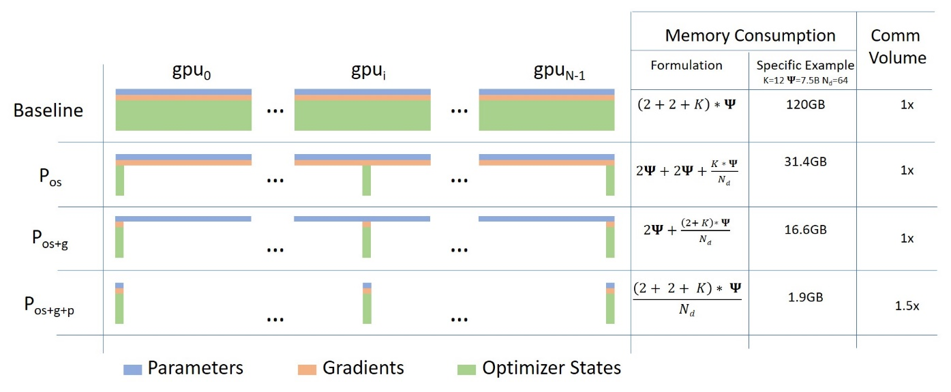
\includegraphics[width=1.0\textwidth]{deepspeed_zero.png}
    \captionof{figure}{So sánh việc sử dụng bộ nhớ trong Data Parallelism tiêu chuẩn và các giai đoạn của ZeRO. ZeRO giảm đáng kể sự thừa thãi bằng cách phân mảnh các thành phần của quá trình huấn luyện.}
    \label{fig:deepspeed_zero}
\end{center}

\paragraph{Tích hợp DeepSpeed với `Trainer`}
Sức mạnh của hệ sinh thái Hugging Face là việc tích hợp các công cụ phức tạp này trở nên rất đơn giản.
\begin{enumerate}
    \item \textbf{Tạo file cấu hình DeepSpeed:} Tạo một file JSON (ví dụ: `ds\_config.json`) để định nghĩa các thiết lập bạn muốn sử dụng (ví dụ: bật ZeRO-2, sử dụng precision fp16, thiết lập optimizer).
    \item \textbf{Truyền vào `TrainingArguments`:}
        \begin{tcolorbox}[title=Cấu hình DeepSpeed, colback=black!5!white, colframe=black!80!white]
            \begin{minted}[linenos, numbersep=0pt]{python}
            training_args = TrainingArguments(
                output_dir="./results",
                # ...
                deepspeed="path/to/your/ds_config.json", # Chỉ định file config
            )
            \end{minted}
        \end{tcolorbox}
    \item \textbf{Khởi chạy:} Sử dụng `deepspeed your\_script.py` hoặc `accelerate launch --use\_deepspeed your\_script.py` để chạy kịch bản.
\end{enumerate}
`Trainer` và `accelerate` sẽ tự động xử lý tất cả các chi tiết phức tạp của việc khởi tạo và chạy DeepSpeed.

Ngoài ZeRO, DeepSpeed còn cung cấp nhiều tính năng tối ưu hóa khác như \textbf{Offloading} (chuyển bớt các tham số không dùng đến từ VRAM sang CPU RAM hoặc NVMe) và các kernel hiệu năng cao. Bằng cách kết hợp các công cụ như `accelerate` và `DeepSpeed`, việc huấn luyện các mô hình ngôn ngữ lớn không còn là đặc quyền của một vài phòng thí nghiệm AI lớn, mà đã trở nên dễ tiếp cận hơn với cộng đồng nghiên cứu và các doanh nghiệp.

\bigskip
\hrule
\bigskip

\begin{center}
    \textbf{\Large KẾT THÚC CHƯƠNG 2}
\end{center}

\textit{Chương 2 đã trang bị cho bạn một bộ công cụ thực chiến hoàn chỉnh, từ việc làm quen với hệ sinh thái Hugging Face, xây dựng các quy trình đánh giá đáng tin cậy, đến việc quản lý các thí nghiệm một cách khoa học và huấn luyện các mô hình trên quy mô lớn. Với những kỹ năng này, bạn đã sẵn sàng để đối mặt với những thách thức phức tạp hơn trong việc triển khai và vận hành các hệ thống NLP trong môi trường production, chủ đề của chương tiếp theo.}